\documentclass[]{book}
\usepackage{lmodern}
\usepackage{amssymb,amsmath}
\usepackage{ifxetex,ifluatex}
\usepackage{fixltx2e} % provides \textsubscript
\ifnum 0\ifxetex 1\fi\ifluatex 1\fi=0 % if pdftex
  \usepackage[T1]{fontenc}
  \usepackage[utf8]{inputenc}
\else % if luatex or xelatex
  \ifxetex
    \usepackage{mathspec}
  \else
    \usepackage{fontspec}
  \fi
  \defaultfontfeatures{Ligatures=TeX,Scale=MatchLowercase}
\fi
% use upquote if available, for straight quotes in verbatim environments
\IfFileExists{upquote.sty}{\usepackage{upquote}}{}
% use microtype if available
\IfFileExists{microtype.sty}{%
\usepackage{microtype}
\UseMicrotypeSet[protrusion]{basicmath} % disable protrusion for tt fonts
}{}
\usepackage[margin=1in]{geometry}
\usepackage{hyperref}
\hypersetup{unicode=true,
            pdftitle={StatPREP: Instructor Notes},
            pdfauthor={Daniel Kaplan},
            pdfborder={0 0 0},
            breaklinks=true}
\urlstyle{same}  % don't use monospace font for urls
\usepackage{natbib}
\bibliographystyle{apalike}
\usepackage{color}
\usepackage{fancyvrb}
\newcommand{\VerbBar}{|}
\newcommand{\VERB}{\Verb[commandchars=\\\{\}]}
\DefineVerbatimEnvironment{Highlighting}{Verbatim}{commandchars=\\\{\}}
% Add ',fontsize=\small' for more characters per line
\usepackage{framed}
\definecolor{shadecolor}{RGB}{248,248,248}
\newenvironment{Shaded}{\begin{snugshade}}{\end{snugshade}}
\newcommand{\KeywordTok}[1]{\textcolor[rgb]{0.13,0.29,0.53}{\textbf{#1}}}
\newcommand{\DataTypeTok}[1]{\textcolor[rgb]{0.13,0.29,0.53}{#1}}
\newcommand{\DecValTok}[1]{\textcolor[rgb]{0.00,0.00,0.81}{#1}}
\newcommand{\BaseNTok}[1]{\textcolor[rgb]{0.00,0.00,0.81}{#1}}
\newcommand{\FloatTok}[1]{\textcolor[rgb]{0.00,0.00,0.81}{#1}}
\newcommand{\ConstantTok}[1]{\textcolor[rgb]{0.00,0.00,0.00}{#1}}
\newcommand{\CharTok}[1]{\textcolor[rgb]{0.31,0.60,0.02}{#1}}
\newcommand{\SpecialCharTok}[1]{\textcolor[rgb]{0.00,0.00,0.00}{#1}}
\newcommand{\StringTok}[1]{\textcolor[rgb]{0.31,0.60,0.02}{#1}}
\newcommand{\VerbatimStringTok}[1]{\textcolor[rgb]{0.31,0.60,0.02}{#1}}
\newcommand{\SpecialStringTok}[1]{\textcolor[rgb]{0.31,0.60,0.02}{#1}}
\newcommand{\ImportTok}[1]{#1}
\newcommand{\CommentTok}[1]{\textcolor[rgb]{0.56,0.35,0.01}{\textit{#1}}}
\newcommand{\DocumentationTok}[1]{\textcolor[rgb]{0.56,0.35,0.01}{\textbf{\textit{#1}}}}
\newcommand{\AnnotationTok}[1]{\textcolor[rgb]{0.56,0.35,0.01}{\textbf{\textit{#1}}}}
\newcommand{\CommentVarTok}[1]{\textcolor[rgb]{0.56,0.35,0.01}{\textbf{\textit{#1}}}}
\newcommand{\OtherTok}[1]{\textcolor[rgb]{0.56,0.35,0.01}{#1}}
\newcommand{\FunctionTok}[1]{\textcolor[rgb]{0.00,0.00,0.00}{#1}}
\newcommand{\VariableTok}[1]{\textcolor[rgb]{0.00,0.00,0.00}{#1}}
\newcommand{\ControlFlowTok}[1]{\textcolor[rgb]{0.13,0.29,0.53}{\textbf{#1}}}
\newcommand{\OperatorTok}[1]{\textcolor[rgb]{0.81,0.36,0.00}{\textbf{#1}}}
\newcommand{\BuiltInTok}[1]{#1}
\newcommand{\ExtensionTok}[1]{#1}
\newcommand{\PreprocessorTok}[1]{\textcolor[rgb]{0.56,0.35,0.01}{\textit{#1}}}
\newcommand{\AttributeTok}[1]{\textcolor[rgb]{0.77,0.63,0.00}{#1}}
\newcommand{\RegionMarkerTok}[1]{#1}
\newcommand{\InformationTok}[1]{\textcolor[rgb]{0.56,0.35,0.01}{\textbf{\textit{#1}}}}
\newcommand{\WarningTok}[1]{\textcolor[rgb]{0.56,0.35,0.01}{\textbf{\textit{#1}}}}
\newcommand{\AlertTok}[1]{\textcolor[rgb]{0.94,0.16,0.16}{#1}}
\newcommand{\ErrorTok}[1]{\textcolor[rgb]{0.64,0.00,0.00}{\textbf{#1}}}
\newcommand{\NormalTok}[1]{#1}
\usepackage{longtable,booktabs}
\usepackage{graphicx,grffile}
\makeatletter
\def\maxwidth{\ifdim\Gin@nat@width>\linewidth\linewidth\else\Gin@nat@width\fi}
\def\maxheight{\ifdim\Gin@nat@height>\textheight\textheight\else\Gin@nat@height\fi}
\makeatother
% Scale images if necessary, so that they will not overflow the page
% margins by default, and it is still possible to overwrite the defaults
% using explicit options in \includegraphics[width, height, ...]{}
\setkeys{Gin}{width=\maxwidth,height=\maxheight,keepaspectratio}
\IfFileExists{parskip.sty}{%
\usepackage{parskip}
}{% else
\setlength{\parindent}{0pt}
\setlength{\parskip}{6pt plus 2pt minus 1pt}
}
\setlength{\emergencystretch}{3em}  % prevent overfull lines
\providecommand{\tightlist}{%
  \setlength{\itemsep}{0pt}\setlength{\parskip}{0pt}}
\setcounter{secnumdepth}{5}
% Redefines (sub)paragraphs to behave more like sections
\ifx\paragraph\undefined\else
\let\oldparagraph\paragraph
\renewcommand{\paragraph}[1]{\oldparagraph{#1}\mbox{}}
\fi
\ifx\subparagraph\undefined\else
\let\oldsubparagraph\subparagraph
\renewcommand{\subparagraph}[1]{\oldsubparagraph{#1}\mbox{}}
\fi

%%% Use protect on footnotes to avoid problems with footnotes in titles
\let\rmarkdownfootnote\footnote%
\def\footnote{\protect\rmarkdownfootnote}

%%% Change title format to be more compact
\usepackage{titling}

% Create subtitle command for use in maketitle
\newcommand{\subtitle}[1]{
  \posttitle{
    \begin{center}\large#1\end{center}
    }
}

\setlength{\droptitle}{-2em}
  \title{StatPREP: Instructor Notes}
  \pretitle{\vspace{\droptitle}\centering\huge}
  \posttitle{\par}
  \author{Daniel Kaplan}
  \preauthor{\centering\large\emph}
  \postauthor{\par}
  \predate{\centering\large\emph}
  \postdate{\par}
  \date{2018-06-06}

\usepackage{booktabs}
\usepackage{amsthm}
\makeatletter
\def\thm@space@setup{%
  \thm@preskip=8pt plus 2pt minus 4pt
  \thm@postskip=\thm@preskip
}
\makeatother

\usepackage{amsthm}
\newtheorem{theorem}{Theorem}[chapter]
\newtheorem{lemma}{Lemma}[chapter]
\theoremstyle{definition}
\newtheorem{definition}{Definition}[chapter]
\newtheorem{corollary}{Corollary}[chapter]
\newtheorem{proposition}{Proposition}[chapter]
\theoremstyle{definition}
\newtheorem{example}{Example}[chapter]
\theoremstyle{definition}
\newtheorem{exercise}{Exercise}[chapter]
\theoremstyle{remark}
\newtheorem*{remark}{Remark}
\newtheorem*{solution}{Solution}
\begin{document}
\maketitle

{
\setcounter{tocdepth}{1}
\tableofcontents
}
\chapter{Pocket guide to StatPREP
commands}\label{pocket-guide-to-statprep-commands}

\begin{figure}
\centering
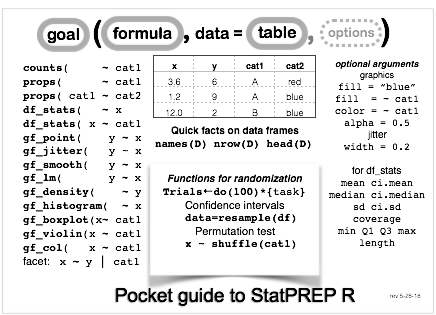
\includegraphics{images/essential_statprep_commands.png}
\caption{}
\end{figure}

\chapter{Signing up for cloud
services}\label{signing-up-for-cloud-services}

You don't need to install any special software on your own computer.
Instead, we'll use services in the cloud that work through a standard
web browser.

It's helpful if you set up a personal account on the cloud services
listed below. That will save time on the day of the workshop and you can
be a resource for your neighbor if they haven't had a chance to do so.
(Do remember to keep track of your user ID and password. Writing it down
is a good idea; you can chance the password after the workshop if you
are worried about security.)

\section{Google}\label{google}

You may already have a Google account: many people have an account
already or work at an institution that provides email and other services
through Google. If so, you are all set.

If you don't already have an account, follow
\href{https://support.google.com/mail/answer/56256?hl=en}{this link to
sign up}.

Setting up a Google account is entirely to streamline authentication to
other services that we use with StatPREP. You do not need to change
anything about your existing email service or how you use it.

\section{GitHub}\label{github}

Funny name, huh? GitHub is a free service with tens of millions of
users. It's most closely associated with software development, but our
main use for it will be to give you a way easily to create a web page to
give your classes access to whichever StatPREP tutorials, lessons, or
Little Apps you choose to use with them.

Your institution may already provide you with a web site or a system
such as Moodle or Blackboard that gives you a class-specific web page.
If so, the point of setting up a GitHub account to use at the workshop
is to make it easier for us to avoid having to figure out how to upload
documents to a multiplicity of different web platforms.

In selecting your user ID for GitHub, keep in mind that the ID is
something that will be visible to students. So, \texttt{ProfJones} or
something of that kind is probably better than
\texttt{Red\_hot\_pepper\_dude}.

Follow \href{https://github.com/}{this link to GitHub's account creation
page}. And \emph{don't be intimidated} by the ``Built for developers''
label.

Once you've set up your account, GitHub will email a confirmation
letter. \textbf{Make sure to click the confirm button} in the email.

\section{RStudio cloud}\label{rstudio-cloud}

We want you to have access to RStudio so that you can use it \emph{if
you decide you want to}. We'll show everyone some basics at the workshop
so you can make an informed decision.

You can sign in using either your Google or your GitHub credentials;
there's no need to set up a separate ID or password. Go to
\href{rstudio.cloud}{\texttt{rstudio.cloud}}.

\chapter{StatPrep Annie}\label{statprep-annie}

StatPrep Annie is a persona created to depict a real-world StatPREP
instructor who is setting up their statistics course.

\begin{figure}

{\centering 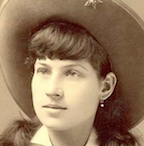
\includegraphics{images/Annie-thumbnail} 

}

\caption{StatPrep Annie}\label{fig:unnamed-chunk-1}
\end{figure}

She's got a website for her course, a couple of interactive lessons, and
so on.

One way to get a quick start on your own website, lessons, etc. is to
copy Annie's project to your own accounts. Then customize it for your
own purposes.

\section{\texorpdfstring{Copying Annie's \texttt{StartUsingR}
project}{Copying Annie's StartUsingR project}}\label{copying-annies-startusingr-project}

\begin{enumerate}
\def\labelenumi{\arabic{enumi}.}
\item
  Using your browser, login to your account on \texttt{rstudio.cloud}.
  The main page for your ``workspace'' will be displayed.
\item
  Open a new tab in the browser. Cut and paste exactly this URL into
  that new tab.

  \texttt{https://rstudio.cloud/project/40418}

  Annie's template will be copied into your workspace. It will open with
  a red ``Temporary'' in the top line.
\item
  Press ``Save a permanent copy'' so that you have your own, fully
  independent copy of Annie's StartUsingR project.
\end{enumerate}

To transform StatPrep Annie's web site to your own, just edit the
\texttt{docs/index.Rmd} file in your copy of the project. Chapter
{[}\#Your\_course\_web\_site{]} shows how to publish the website.

\subsection{Note for those using desktop
RStudio}\label{note-for-those-using-desktop-rstudio}

Copying Annie's \texttt{StartUsingR} project can be done with the ``new
project'' menu in RStudio. Choose to create a new project from a GitHub
repo using this address for cloning:

\begin{verbatim}
https://github.com/StatPrep-Annie/StartingR.git
\end{verbatim}

\section{\texorpdfstring{Editing
\texttt{docs/index.Rmd}}{Editing docs/index.Rmd}}\label{editing-docsindex.rmd}

This will have instructions for editing \texttt{docs/index.Rmd}

\section{Writing your own tutorial}\label{writing-your-own-tutorial}

The file \texttt{tutorials/first-tutorial/first-tutorial.Rmd} has a
template for a tutorial lesson.

\chapter{Your course web site}\label{your-course-web-site}

As statistics instructors start using data in their classes, they find
that they need to make data files available to students. An excellent
way to do that is to put the files on a web site, so that the students
can access them with a URL.

If your institution uses course support software such as Blackboard or
Moodle, you may want to take advantage of those resources.

Many instructors don't have a web server available to them and aren't
sure how to set up a web site. (And, warranted or not, many instructors
grumble about Blackboard and Moodle) The point of this repository is to
help you set up your own course web site on which you can place data
files, etc. so that your students can easily get to them.

\section{Starting point \ldots{}}\label{starting-point}

We'll assume that you have already created an RStudio project, perhaps
simply by copying StatPrep Annie's ``StartUsingR'' project to your own
rstudio.cloud account, as described in Chapter {[}\#StatPrep\_Annie{]}

\section{Creating a GitHub repository for your
project}\label{creating-a-github-repository-for-your-project}

Leaving your RStudio.cloud tab for a few moments, you're going to create
a new repository on GitHub to use for publishing web pages from your
project.

\begin{enumerate}
\def\labelenumi{\arabic{enumi}.}
\item
  Login to GitHub. Once you have done this, access the +v dropdown menu
  in the upper right of the GitHub display:

  \begin{figure}
  \centering
  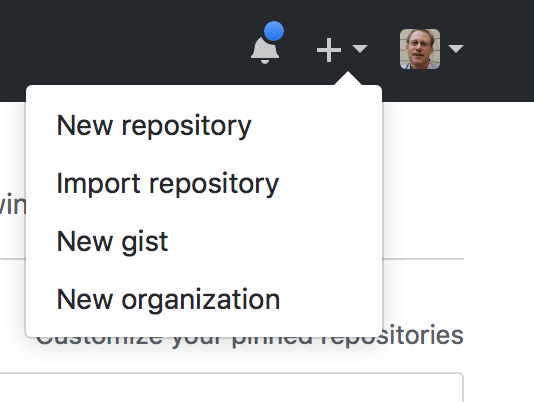
\includegraphics{images/new_repo1.png}
  \caption{}
  \end{figure}

  Select ``new repository''
\item
  In response to your selecting ``new repository,'' GitHub will display
  a set-up page:

  \begin{figure}
  \centering
  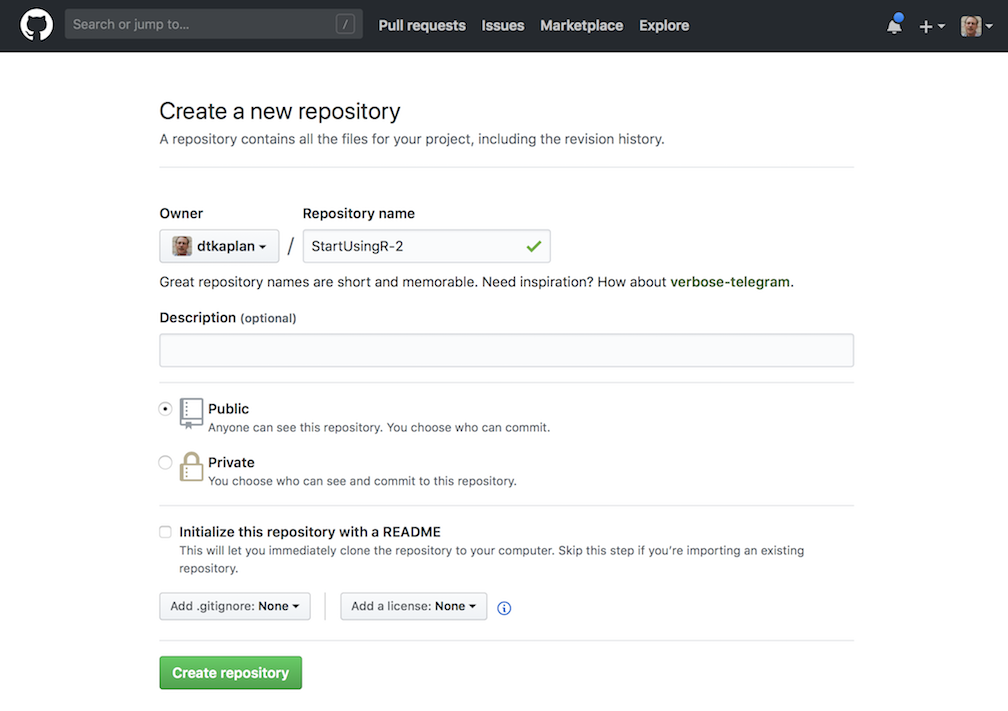
\includegraphics{images/new_repo2.png}
  \caption{}
  \end{figure}

  \begin{itemize}
  \tightlist
  \item
    Choose a suitable name for the repo. For instance, if this is to be
    a course site, you might use the name of the course, e.g.
    \texttt{Stat101}.
  \item
    Once you have set the new repository's name, skip directly on down
    to the green ``Create repository'' button. Press it
  \end{itemize}
\item
  GitHub will now display a ``Quick setup page.'' Near the top will be a
  section that looks like this:

  \begin{figure}
  \centering
  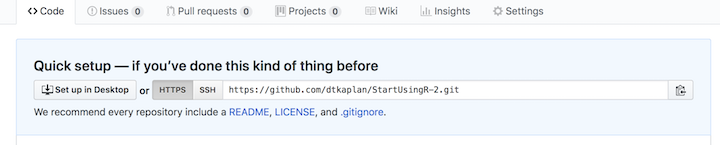
\includegraphics{images/new_repo3.png}
  \caption{}
  \end{figure}
\end{enumerate}

Note the repo URL that appears in the editing box. It is composed from
your GitHub user name and the name you selected for the repository. Keep
that handy. Later, you're going to paste that URL into a command.

\section{Connecting your RStudio project to
GitHub}\label{connecting-your-rstudio-project-to-github}

Your task now is to connect your own copy of the StartUsingR project to
GitHub. To do this, go back to your rstudio.cloud tab displaying your
project.

\begin{enumerate}
\def\labelenumi{\arabic{enumi}.}
\item
  In the Git tab in RStudio, select the ``gear'' menu and then
  ``shell.'' 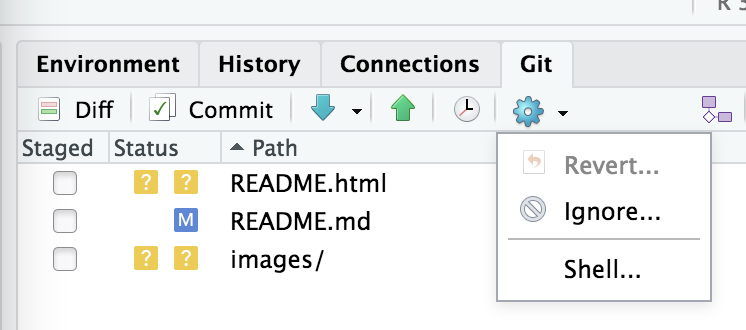
\includegraphics{images/new_repo4.png}

  This will open up a new tab called ``Terminal'', next to the console.
\item
  In the Terminal tab, cut and paste these commands, making sure to
  \textbf{provide your own email address and name} rather than StatPrep
  Annie's. (If you have multiple email addresses, or multiple names, you
  can use any of them!)

\begin{Shaded}
\begin{Highlighting}[]
\NormalTok{git config }\OperatorTok{--}\NormalTok{global user.email }\StringTok{"StatPrep.Annie@gmail.com"}
\NormalTok{git config }\OperatorTok{--}\NormalTok{global user.name }\StringTok{"StatPrep Annie"}
\end{Highlighting}
\end{Shaded}

  Press enter. There will be no response by the computer. You're going
  to be using the terminal tab later, as well.
\item
  Give the command, in the terminal tab, that will instruct RStudio to
  refer to your GitHub repository. The command will look like the
  following, but \textbf{you must} change \texttt{USERNAME} to be your
  own GitHub username, and change \texttt{REPOSITORY} to be your own
  repository, set up in Step (1) of this section.

\begin{verbatim}
git remote set-url origin <paste_your_repo_URL_here>
\end{verbatim}

  Again, when you press ``enter'', the computer will not respond.
\item
  In RStudio, open up some file, say, \texttt{README.Rmd}, and make some
  trivial change, such as adding a space after the document title. Then
  save the file.
\item
  In RStudio, go to the Git tab. You will see the name of the file you
  just edited (and maybe some others). Check the little box under
  ``Staged'' to the left of the file name. Then, press Commit.
\item
  A new window will open that looks like a bigger version of the Git
  tab.

  \begin{figure}
  \centering
  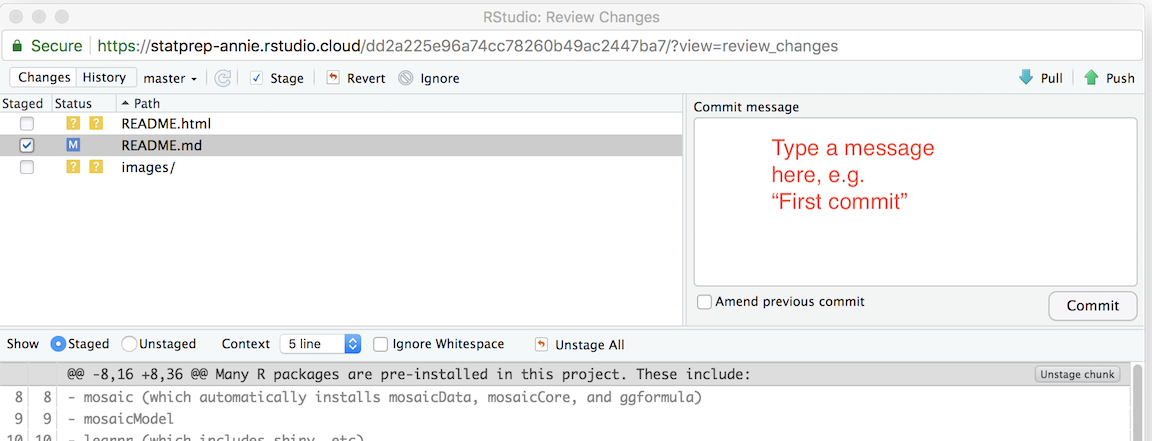
\includegraphics{images/new_repo6.png}
  \caption{}
  \end{figure}

  Write some short message in the box and press the ``commit'' button
  underneath the message box.
\item
  Almost done \ldots{} Press the green upward pointing arrow above the
  message box. You will be prompted to enter your GitHub account ID and
  password. Do so.
\item
  Now back to your GitHub account. Go to the repository you set up and
  press ``settings.'' Under gh-pages in settings, select ``master branch
  docs folder.'' In response, a github.io URL will appear in the
  gh-pages section. That's the address of the web site.
\end{enumerate}

In a few minutes, you should be able to access your new web page using
your own GitHub.io address.

\subsubsection{Putting links to data files on your own course web
site}\label{putting-links-to-data-files-on-your-own-course-web-site}

If you are going to use your site to provide student access to data sets
of particular interest to you, you will want to put links and
instructions on your course web site.

The markup that you include in your \texttt{index.md} file (in the
\texttt{docs/} directory) might look like this:

\begin{verbatim}
## Google files used in class

- `Survey1 <- gs_read(gs_key("1ucevNh7wKLtOukyEpacUKi5_-KZUQGtIOONhWRnnnQ4"))`

## Data files

Data files for this week:

- `https://dtkaplan.github.io/stat101/test.csv`

To create the data table in your R session, copy and paste 
this command into your console:

```r
My_data <- read.csv("https://dtkaplan.github.io/stat101/test.csv")
```
\end{verbatim}

\subsection{Customizing your site with
RStudio}\label{customizing-your-site-with-rstudio}

Outline:

\begin{itemize}
\tightlist
\item
  clone the repo
\item
  open a new project in RStudio, choosing the option for a GitHub
  repository.
\item
  Edit as needed. Every file you edit should be ``knitted'' to HTML.
\item
  State, commit, push, and pull.
\end{itemize}

\chapter{Class data using Google
Sheets}\label{class-data-using-google-sheets}

Collecting data interactively with students has several benefits:

\begin{enumerate}
\def\labelenumi{\arabic{enumi}.}
\tightlist
\item
  Students see the connection between the data and their own actions.
  Students are especially motivated when the data is about them or
  something they are doing.
\item
  The inevitable imperfections in user-entered data serve as a lesson in
  coding factors and the measuring variables in a standard way.
\item
  The instructor (or individual students) can analyze the data and see
  how the analysis changes in real time, as more data rows are added.
\end{enumerate}

\section{Resources}\label{resources}

Two example lessons, from the StatPREP 2018 Workshops are:

\begin{itemize}
\tightlist
\item
  \href{http://dtkaplan.shinyapps.io/tutorial_globe_toss.png}{Globe
  toss}
\item
  \href{http://dtkaplan.shinyapps.io/Tutorial_Riverboat_shuffle.png}{Riverboat
  card trick}
\end{itemize}

You're welcome to use those interactive documents. Each document has a
link to the spreadsheet for entering data. It's your own choice whether
to start by clearing out any existing rows or add on to the rows from
another session. \textbf{NOTE}: No guarantee that your class's data will
be there later on, since someone else might have erased it. And so you
might want to set up your own spreadsheet exclusively for your class's
use.

The section below on \emph{Setting up a new spreadsheet} shows how to
create a spreadsheet for your class. Note that you should post the link
to your spreadsheet on your course website, so that students can access
it to enter data.

For data analysis, you have a choice of options:

\begin{enumerate}
\def\labelenumi{\arabic{enumi}.}
\tightlist
\item
  Use the
  \href{http://dtkaplan.shinyapps.io/Lesson_read_class_data.png}{Read
  class data} activity. The user will have to paste the command to read
  in your spreadsheet at the start of every command block. (See
  \emph{Setting up a new spreadsheet}.)
\item
  Use your own R session. Again, you will need to give the command to
  read in your spreadsheet into the console.
\item
  Create your own tutorial document in Rmd. This presumes that you are
  comfortable editing Rmd documents and, if you want to give your
  students access, publishing them on a server. A working template is
  available via the StatPREP Workshops2018 project on
  \texttt{rstudio.cloud}.
  (\href{https://rstudio.cloud/project/38547}{Follow this link.} to the
  file \texttt{Google\_data\_template.Rmd}.)
\end{enumerate}

\section{Setting up a new
spreadsheet}\label{setting-up-a-new-spreadsheet}

You can modify this document to work with a spreadsheet of your own.
Here's how.

\begin{enumerate}
\def\labelenumi{\arabic{enumi}.}
\item
  Set up a Google spreadsheet. It's a good idea to populate it with some
  variable names and a few values. This will let you test to make things
  are working before you start the activity in class.
\item
  \emph{Within} the Google spreadsheet document press the ``Share''
  button.

  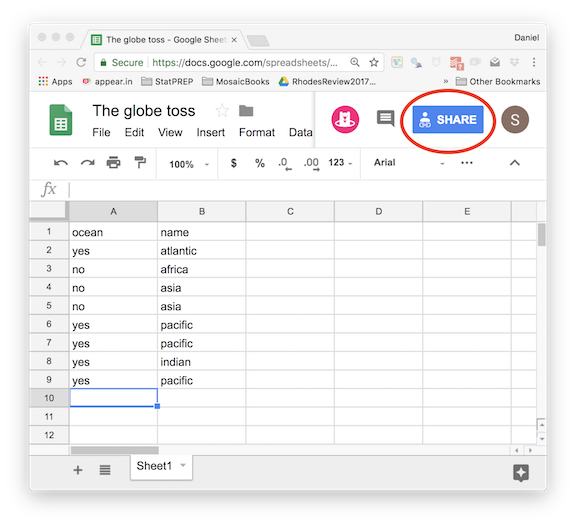
\includegraphics{images/google1.png}
\item
  After you press ``Share,'' you will see a dialog box.

  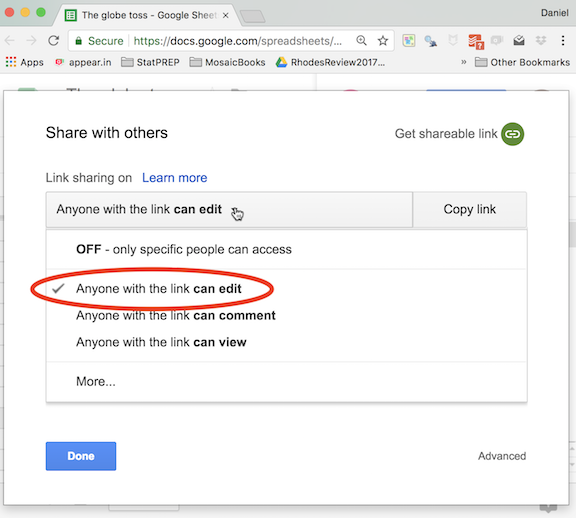
\includegraphics{images/google2.png}

  \begin{itemize}
  \tightlist
  \item
    Pull down the menu to select ``Anyone with the link \textbf{can
    edit}.'' (This is what lets your students add data.)
  \item
    Copy the link and paste it somewhere you can get to it again. You'll
    need it. The link will look like this:
    \texttt{https://docs.google.com/spreadsheets/d/1ucevNh7wKLtOukyEpacUKi5\_-KZUQGtIOONhWRnnnQ4/edit?usp=sharing}
  \item
    You will also need to copy the \emph{key} that's contained in the
    link. The key is just the central gibberish in the link, like this:
    \texttt{1ucevNh7wKLtOukyEpacUKi5\_-KZUQGtIOONhWRnnnQ4}
  \end{itemize}
\item
  Put the link on your course web site so that your students can get to
  it. That's how they will access the spreadsheet for entering data.
\item
  Back in your Google sheet, select the File/Publish\_to\_the\_web menu
  item. Use the resulting dialog box to publish the entire document.
\end{enumerate}

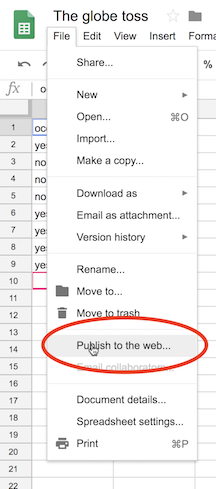
\includegraphics{images/publish1.png}~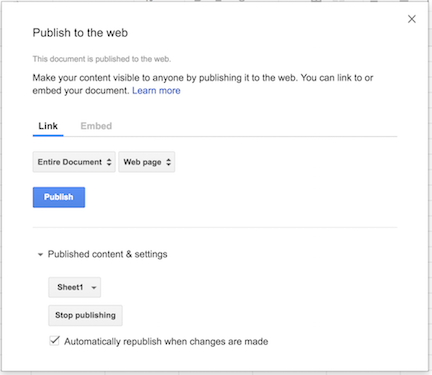
\includegraphics{images/publish2.png}

\begin{enumerate}
\def\labelenumi{\arabic{enumi}.}
\setcounter{enumi}{5}
\item
  Create the R command that will load the spreadsheet data into your R
  session.

\begin{Shaded}
\begin{Highlighting}[]
\NormalTok{Globe <-}\StringTok{ }\KeywordTok{gs_read}\NormalTok{(}\KeywordTok{gs_key}\NormalTok{(}\StringTok{"1ucevNh7wKLtOukyEpacUKi5_-KZUQGtIOONhWRnnnQ4"}\NormalTok{))}
\end{Highlighting}
\end{Shaded}

  In forming the command, replace the quoted string in the above with
  your own key. The key is located in the center of the link to the
  spreadsheet: an incomprehensible set of characters similar to that
  highlighted in \textbf{bold} in the example in step (3). You might
  also replace \texttt{Globe} with a name that's more suited to your own
  activity.

  Paste the command you've created someplace handy. You'll need it.
  (Suggestion: Paste it next to the link in step (4).)
\end{enumerate}

Time for class!

\begin{enumerate}
\def\labelenumi{\arabic{enumi}.}
\setcounter{enumi}{6}
\tightlist
\item
  Once you reach the point in your class where you want to do statistics
  on your data, bring up the lesson document provided for this purpose
  by StatPREP
  \href{http://dtkaplan.shinyapps.io/Lesson_read_class_data.png}{located
  here}. That document has several R command chunks, all of which are
  blank. You can put any R commands in those chunks, \textbf{but make
  sure} that the command from step (5) always is the first command in
  any chunk that you use. That way, whenever you run the code in the
  chunk, the data will be read in from Google. Keep in mind that the
  chunks are all independent of one another, so you'll need to read in
  the data in any chunk you use.
\end{enumerate}

Try it out in the following command chunk:

\begin{enumerate}
\def\labelenumi{\alph{enumi}.}
\tightlist
\item
  Paste in the command you created in step (5).
\item
  Below that, add any R commands you like.
\end{enumerate}

For instructors who want to write their own tutorial, you will find that
this simplifies things since you can arrange to have the spreadsheet
data read-in globally and not have to put the data-reading command in
every chunk. Use the template \texttt{.Rmd} document provided by
StatPREP \href{}{here}. Modify the chunk named \texttt{read\_data} the
top of the document by inserting your own command (with your own key).
Notice that in any new chunk you create, you'll have to reference the
\texttt{read\_data} chunk as the \texttt{exercise-setup}. The chunks
already in the template document do this, so you can just copy (and
rename!) an existing chunk.

\chapter{Using RStudio.cloud}\label{using-rstudio.cloud}

Just some preliminary notes \ldots{}

Under preferences/Rmd, arrange to have the preview opened in the Viewer
tab. It doesn't seem to work to leave it as opening in a web page.

\chapter{Publishing tutorials on
shinyapps.io}\label{publishing-tutorials-on-shinyapps.io}

This chapter is not yet complete.

\section{Authorizing rstudio.cloud to
publish}\label{authorizing-rstudio.cloud-to-publish}

You need to authorize \texttt{rstudio.cloud} to publish to your
\texttt{shinyapps.io} account. How do you do this? The general idea is
that you login to \texttt{shinyapps.io} and ask it to tell you a secret.
Then, from \texttt{rstudio.cloud}, you send that secret back to
\texttt{shinyapps.io}. Once \texttt{shinyapps.io} knows that
\texttt{rstudio.cloud} is in on the secret, shinyapps will accept future
commands from you \texttt{rstudio.cloud} account.

\begin{enumerate}
\def\labelenumi{\arabic{enumi}.}
\tightlist
\item
  Login to your account on \texttt{rstudio.cloud}.
\item
  Open any project on \texttt{rstudio.cloud}.

  \begin{itemize}
  \tightlist
  \item
    From the RStudio interface, select the ``Packages'' tab and press
    ``Install''.
  \end{itemize}

  \begin{center}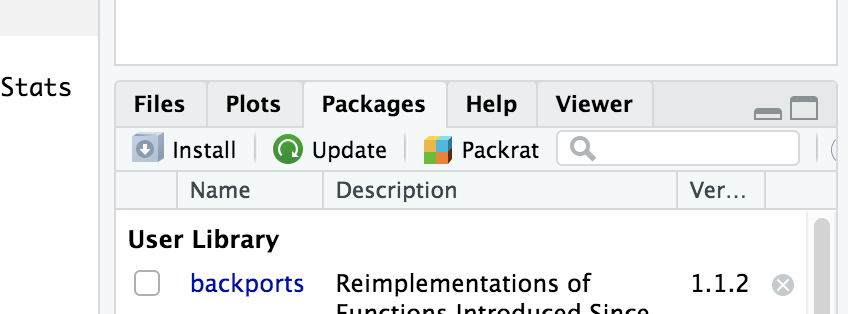
\includegraphics{images/annie-install-rsconnect1} \end{center}

  \begin{itemize}
  \tightlist
  \item
    In the dialog box that appears, start typing \texttt{rsconnect}. At
    some point, the dropdown menu will show that choice. Click on that
    and press ``Install''.
  \end{itemize}
\end{enumerate}

\begin{center}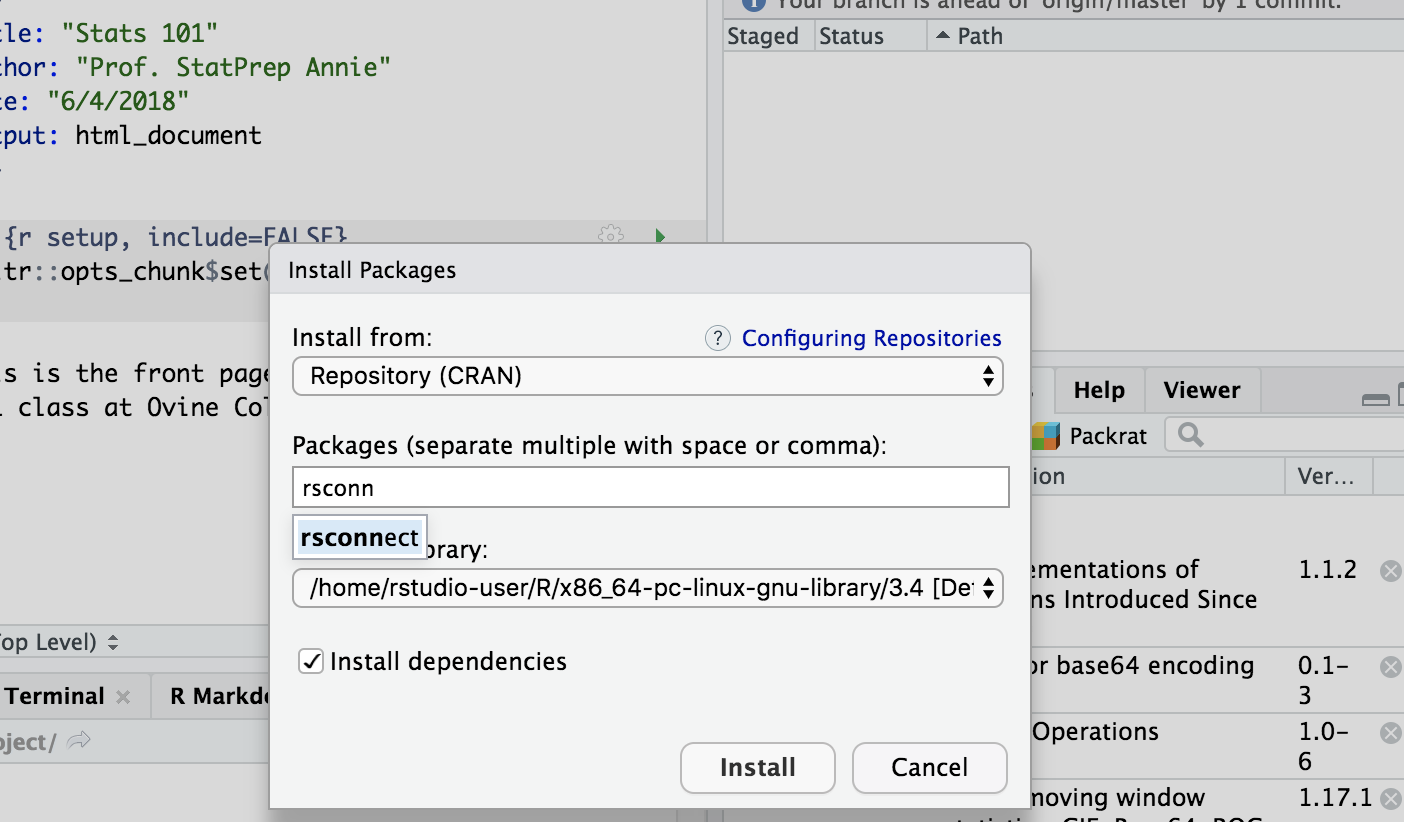
\includegraphics{images/annie-install-rsconnect2} \end{center}

\begin{enumerate}
\def\labelenumi{\arabic{enumi}.}
\setcounter{enumi}{2}
\item
  Login to \texttt{shinyapps.io}. Select the ``Dashboard'' tab. You'll
  see a section entitled ``Authorize account'' with a display of
  computer code and a ``copy to clipboard'' button. Press that button.
  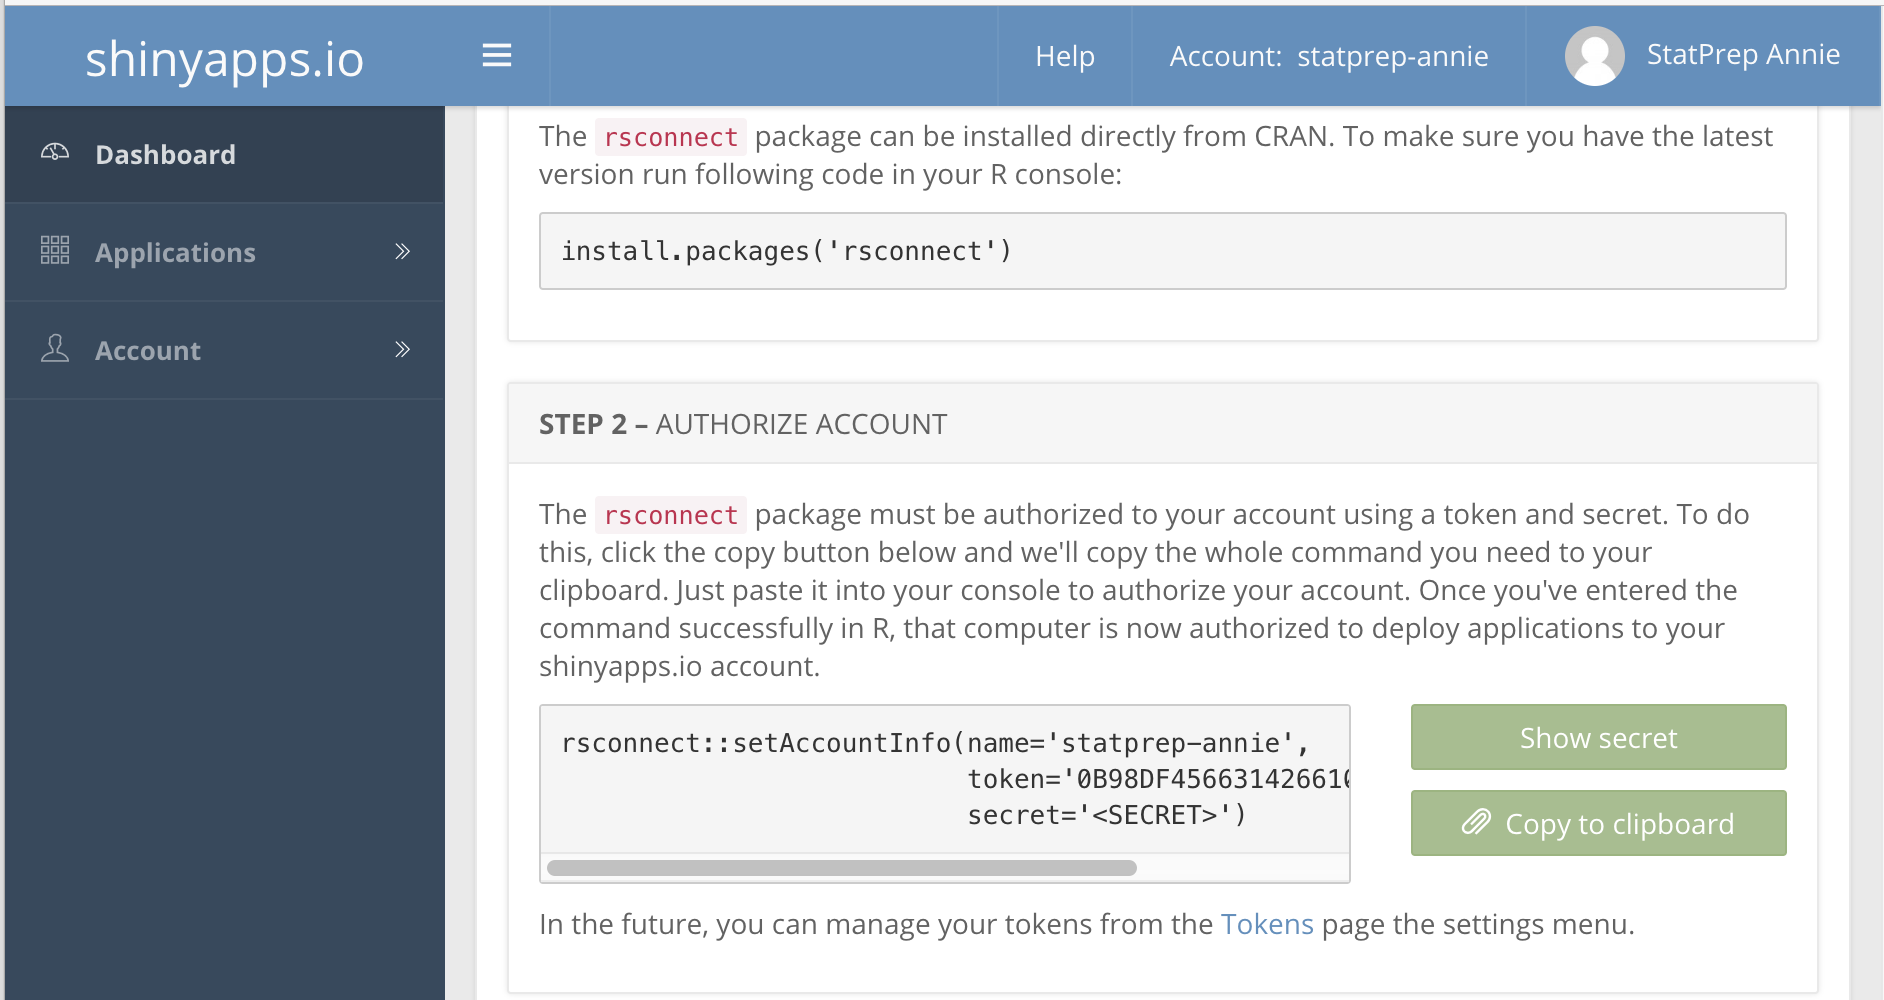
\includegraphics{images/annie-authorize-cloud2.png} Depending on your
  browser, you may be asked to press CNTR-C to copy the code.
\item
  Return to the console in \texttt{rstudio.cloud} and paste in the code
  you copied in (3).
\end{enumerate}

Press the ``Publish'' button. - Select ``RStudio Connect'' - Select
``Publish finished document only'' - In the dialog box titled ``Select
RStudio Connect Account'', type the address \texttt{shinyapps.io}.

\bibliography{book.bib}


\end{document}
